\section{Requirements}

\subsection{User Stories}
\begin{comment}
Use the template from the course website and list all user stories here. It is
fine to have them in an spreadsheet (or other applications, such as Trello) at
first, but they must end up here as well.

These user stories should describe what the user will be able to do. Write
the user stories in language of the customer, and give them a unique ID. List
the user stories in order of priority.

You need to annotate an user story whether or not it is implemented. We need to
know which user stories are implemented, such that we can check this during the
oral presentation.
\end{comment}


\begin{itemize}
	\item \D As an explorer i want to be able to to move around in the world so i can see new places
	      \begin{itemize}[+]
		      \item Change location of player character.
		      \item Take input from player.
		      \item Move player according to input.
		      \item Animation when walking.
		      \item Animation when standing still.
	      \end{itemize}
	\item \D As an explorer i want to be able to transition between different maps, so that i'm not stuck in the same area
	      \begin{itemize}[+]
		      \item Update Map not to be static and use a map manager instead
		      \item Do the same thing as above for texture map
		      \item Create multiple maps
		      \item Update parser to use map transition data
		      \item Transition logically
		      \item Make TextureMapManager observe model MapManager for changing map
	      \end{itemize}
	\item \D As a pacifist I want to be able to run from combat so my monsters don't get hurt
	      \begin{itemize}[+]
		      \item Run action in combat menu
		      \item Chance to end combat when running away
	      \end{itemize}
	\item \D As a player i want to see my environment so I know where I am
	      \begin{itemize}[+]
		      \item Parse tile sets.
		      \item Implement map renderer class
	      \end{itemize}
	\item \D As a player i want my monsters to be able to attack, so I can win against other monsters.
	      \begin{itemize}[+]
		      \item Create an attack handler witch handles attacks
		      \item Create a way for monsters to take damage
	      \end{itemize}
	\item \D As a player i want the game to understand my inputs so i can play the game
	      \begin{itemize}[+]
		      \item Implement an input listener
		      \item Make input listener take input from keyboard
		      \item Connect Input to model
	      \end{itemize}
	\item \D As a modder, i want to be able to parse and make my own Tiled maps
	      \begin{itemize}[+]
		      \item Load tile sets from Tiled file
		      \item Load tile information from Tiled file
	      \end{itemize}
	\item \D as a player, I want to be able to fine a monster to attack
	      \begin{itemize}[+]
		      \item Encounters to trigger a new combat
		      \item Change scene to view combat
	      \end{itemize}
	\item \D As a realist I want the world to limit my movements so I cant't walk through walls
	      \begin{itemize}[+]
		      \item Implement collision logic
		      \item Parse collision from a map file
	      \end{itemize}
	\item \D As a player i want to be able to attack a monster with my monster because i want to be able to win
	      \begin{itemize}[+]
		      \item Design health interface
		      \item Implement health interface
		      \item implement hit enemy.
	      \end{itemize}
	\item As a collector I want to keep multiple monster with me so that I can use more then one
	      \begin{itemize}[+]
		      \item Implement somewhere to store multiple monsters
		      \item Design an interface for seeing your monsters
		      \item Pick one that is the current one
	      \end{itemize}
	\item As a pacifist, I want to befriend my enemies so I can have more friends
	      \begin{itemize}[+]
		      \item Design a befriend interface
		      \item Add befriending difficulty to monsters
		      \item Display befriending difficulty in combat
		      \item Add befriended monster to you monster party
	      \end{itemize}
	\item As a player, I want to be able to pick an attack so that I can strategically control my monster during combat
	      \begin{itemize}[+]
		      \item Design a "pick an attack"- interface
		      \item Implement visuals fo said interface
		      \item Create several (more then one) different attacks to choice from
	      \end{itemize}
	\item As a speedrunner
	      \begin{itemize}[+]
		      \item Design a befriend interface
		      \item Add befriending difficulty to monsters
		      \item Display befriending difficulty in combat
		      \item Add befriended monster to you monster party
	      \end{itemize}
\end{itemize}



\subsection{Definition of Done}
\begin{comment}
In this section you list the acceptance criteria that are common for all user
stories. For example, the code should reviewed and tests, it should be under
version control, etc.
\end{comment}
The project code was structured in such a way that when a person felt that they were done with a user story, they had to get it reviewed and be questioned about it by at least one other contributor. The purpose of this practice was not only to make sure that the user story was implemented fully, that can be done with tests, but to iron out code smells and to keep the code somewhat coherent and similar-looking throughout the project.

\subsection{User interface}
\begin{comment}
Include sketches, drawings and explanations of the application's user interface.
Describe the navigation between the different views.
\end{comment}
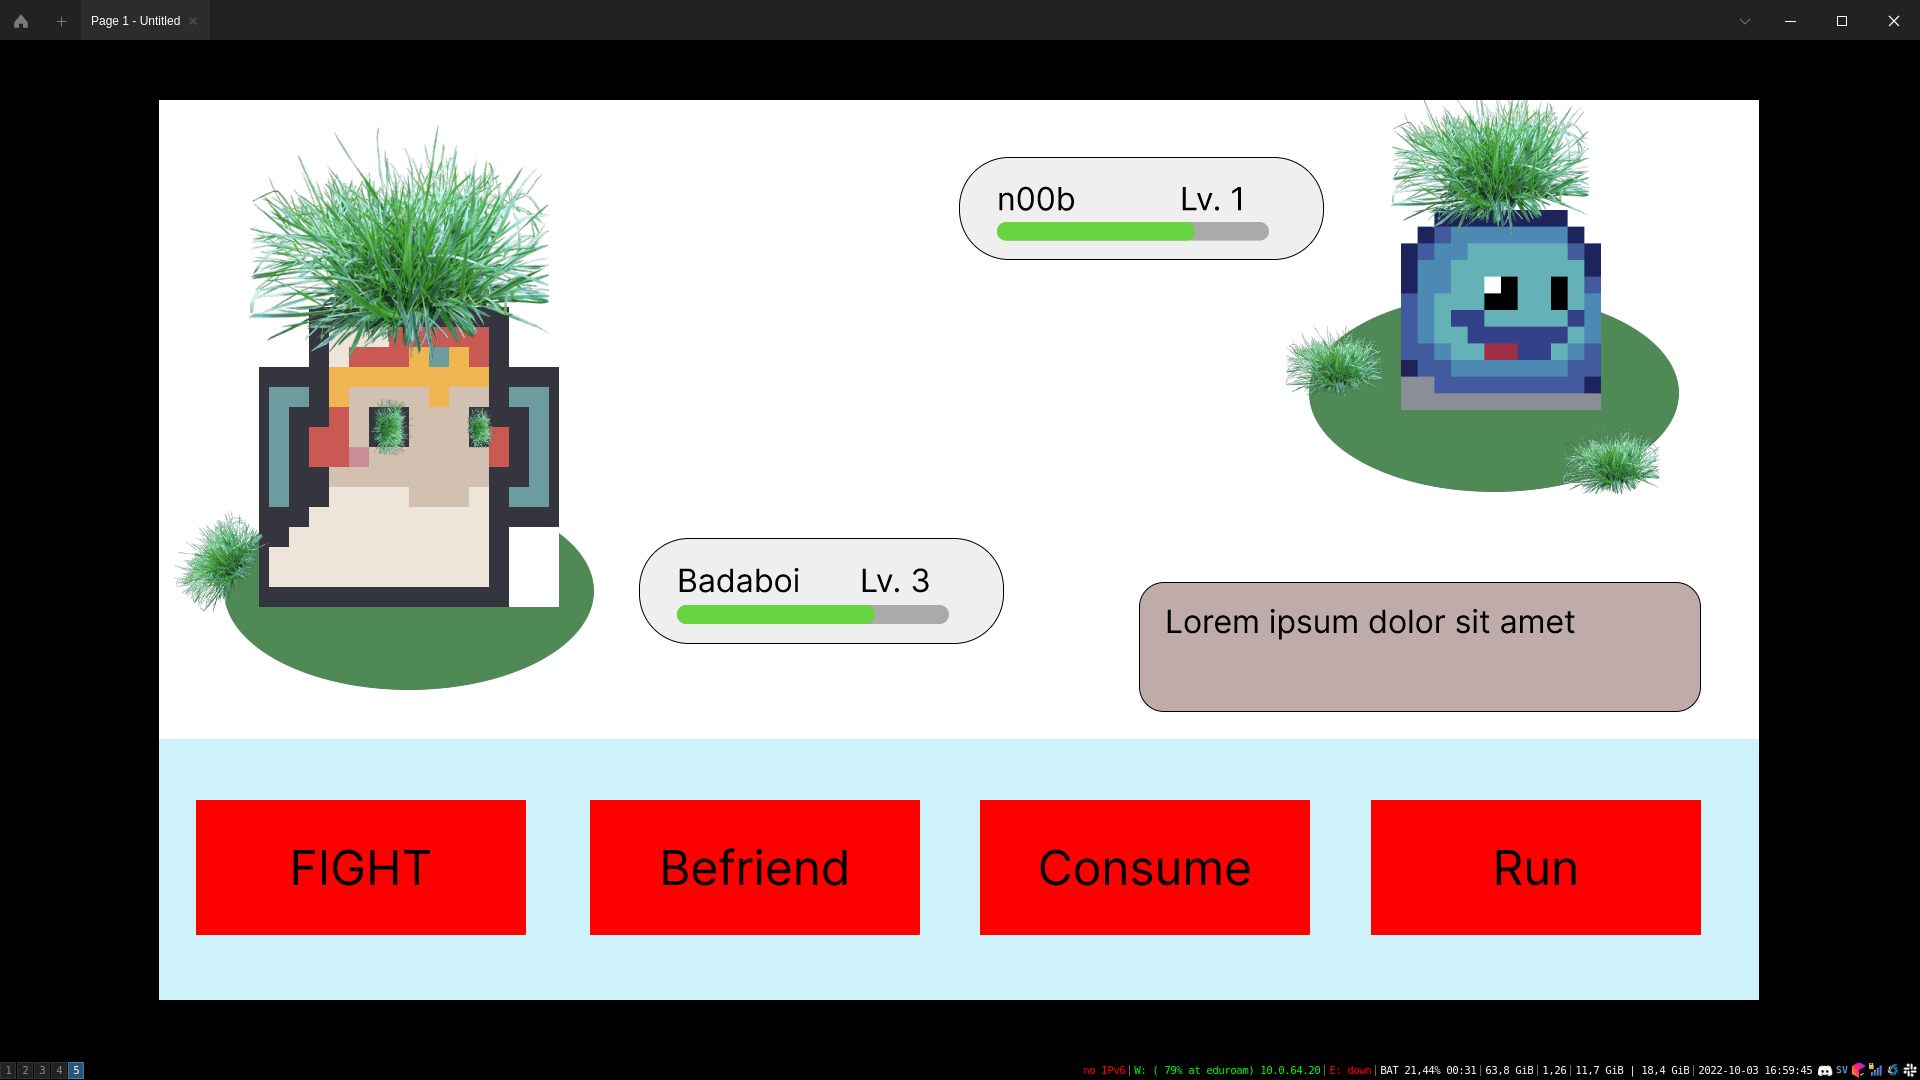
\includegraphics[width=\textwidth]{images/combat_figma.png}